\documentclass{article}

% supress page numbering so that a single eps figure can be generated:
\usepackage{nopageno}

\usepackage{tikz}
\usetikzlibrary{bayesnet}

\begin{document}

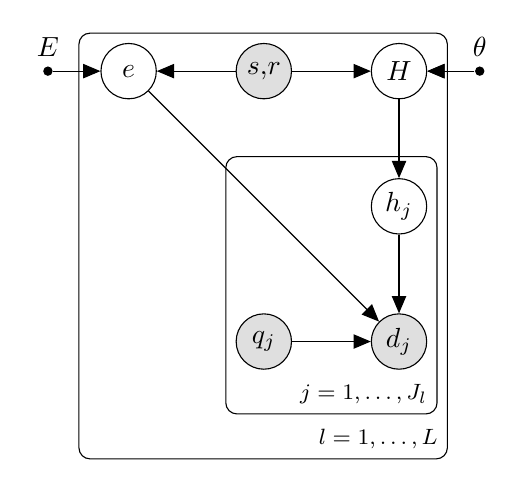
\begin{tikzpicture}
  \node[obs] (dj) {$d_j$} ;
  \node[obs, left=of dj] (qj) {$q_j$} ;
  \node[latent, above=of dj] (hj) {$h_j$} ;
  \node[latent, above=of hj] (H) {$H$} ;
  \node[obs, left=of H] (sr) {$s$,$r$} ;
  \node[latent, left=of sr] (e) {$e$} ;
  \node[left=-0.1 of e] (plateSpace) {};
  \node[above=-0.1 of hj] (jplateSpace) {};
  \node[circle,fill,inner sep=1.2pt, right=0.6 of H, label=above:\fontsize{10}{10}\selectfont$\theta$] (theta) {};
  \node[circle,fill,inner sep=1.2pt, left=0.6 of e, label=above:\fontsize{10}{10}\selectfont$E$] (E) {};
  \edge {qj,hj,e} {dj} ;
  \edge {H} {hj} ;
  \edge {sr,theta} {H} ;
  \edge {sr,E} {e} ;
  \edge {theta} {H}
  \plate {jplate} {(dj)(qj)(hj)(jplateSpace)} {$j = 1,\ldots,J_l$}
  \plate {lplate} {(dj)(qj)(hj)(H)(sr)(e)(plateSpace)(jplate.south east)} {$l = 1,\ldots,L$}
\end{tikzpicture}

\end{document}
